% Created 2018-04-21 Sat 02:51
% Intended LaTeX compiler: pdflatex
\documentclass[bigger,unknownkeysallowed]{beamer}
\usepackage[utf8]{inputenc}
\usepackage[T1]{fontenc}
\usepackage{graphicx}
\usepackage{grffile}
\usepackage{longtable}
\usepackage{wrapfig}
\usepackage{rotating}
\usepackage[normalem]{ulem}
\usepackage{amsmath}
\usepackage{textcomp}
\usepackage{amssymb}
\usepackage{capt-of}
\usepackage{hyperref}
\usepackage{xcolor}
\usepackage{listings}
\titlegraphic{
\includegraphics{ccbysa.png}}
\lstset{escapeinside={'}{'},basicstyle=\scriptsize\ttfamily,showspace=false}
\usetheme{ucadoc}
\author{Daniel Molina Cabrera}
\date{Curso de Python (Abril 2018)}
\title{Casos de uso de Python}
\hypersetup{
 pdfauthor={Daniel Molina Cabrera},
 pdftitle={Casos de uso de Python},
 pdfkeywords={},
 pdfsubject={},
 pdfcreator={Emacs 25.1.1 (Org mode 9.1.9)}, 
 pdflang={English}}
\begin{document}

\maketitle
\AtBeginSection[]{ \begin{frame}{Índice}     \tableofcontents     \end{frame} }
\section{}
\label{sec:orgd214080}

\begin{frame}[label={sec:orgb1da1c2}]{Casos de uso de Python}
\begin{center}
\begin{center}

\includegraphics[width=.7\textwidth]{when.png}
\end{center}
\end{center}


\begin{columns}
\begin{column}{0.4\columnwidth}
\begin{center}
\begin{center}

\includegraphics[width=\textwidth]{python_inside.jpg}
\end{center}
\end{center}
\end{column}
\begin{column}{0.6\columnwidth}
\begin{block}{Qué veremos}
\begin{itemize}
\item Áreas donde Python aporta.

\item Librerías recomendadas.
\end{itemize}
\end{block}
\end{column}
\end{columns}
\end{frame}

\begin{frame}[label={sec:orgc2c4850}]{Áreas que veremos}
\begin{center}
\begin{center}

\includegraphics[width=.6\textwidth]{sciencevsweb.png}
\end{center}
\end{center}

\begin{columns}
\begin{column}{0.5\columnwidth}
\begin{block}{Ciencia}
\begin{itemize}
\item Cálculo: Numpy, Pandas.

\item Visualización.
\end{itemize}
\end{block}
\end{column}

\begin{column}{0.5\columnwidth}
\begin{block}{Programación web}
\begin{itemize}
\item Backend: Django, Flask.
\end{itemize}
\end{block}
\end{column}
\end{columns}
\end{frame}


\section{Python para la ciencia}
\label{sec:org51c8c0c}

\begin{frame}[label={sec:orga7ba136}]{Python para la ciencia}
\begin{center}
\begin{center}

\includegraphics[width=0.6\textwidth]{python_science.png}
\end{center}
\end{center}

\begin{block}{Python para la ciencia}
\begin{itemize}
\item Python se usa mucho para la ciencia de datos\footnote{\url{http://awahid.net/blog/data-science-with-python-or-java/}}.

\item Gran parte de su comunidad son científicos, no informáticos.
\end{itemize}
\end{block}
\end{frame}


\begin{frame}[label={sec:orgc96da70}]{¿Qué aporta Python en la ciencia?}
\begin{block}{Ventajas}
\begin{itemize}
\item Lenguaje fácil de usar para no informáticos.

\item Comunidad amigable.

\item Librerías científicas avanzadas fáciles de usar.

\item Entorno desarrollo estable.

\item Paralelismo.
\end{itemize}
\end{block}
\end{frame}

\begin{frame}[label={sec:orgc030f8b}]{Utilidad de Python}
Utilidad en proceso científico \footnote{\url{https://www.slideshare.net/marcelcaraciolo/computao-cientfica-com-python-numpy-e-scipy}\label{org71116df}} 
\begin{center}
\includegraphics<1>[width=.6\textwidth]{fases.png}
\includegraphics<2>[width=.6\textwidth]{python_fases.png}
\end{center}
\end{frame}


\begin{frame}[label={sec:org21c85de}]{Uso de Python}
\begin{center}
\begin{center}
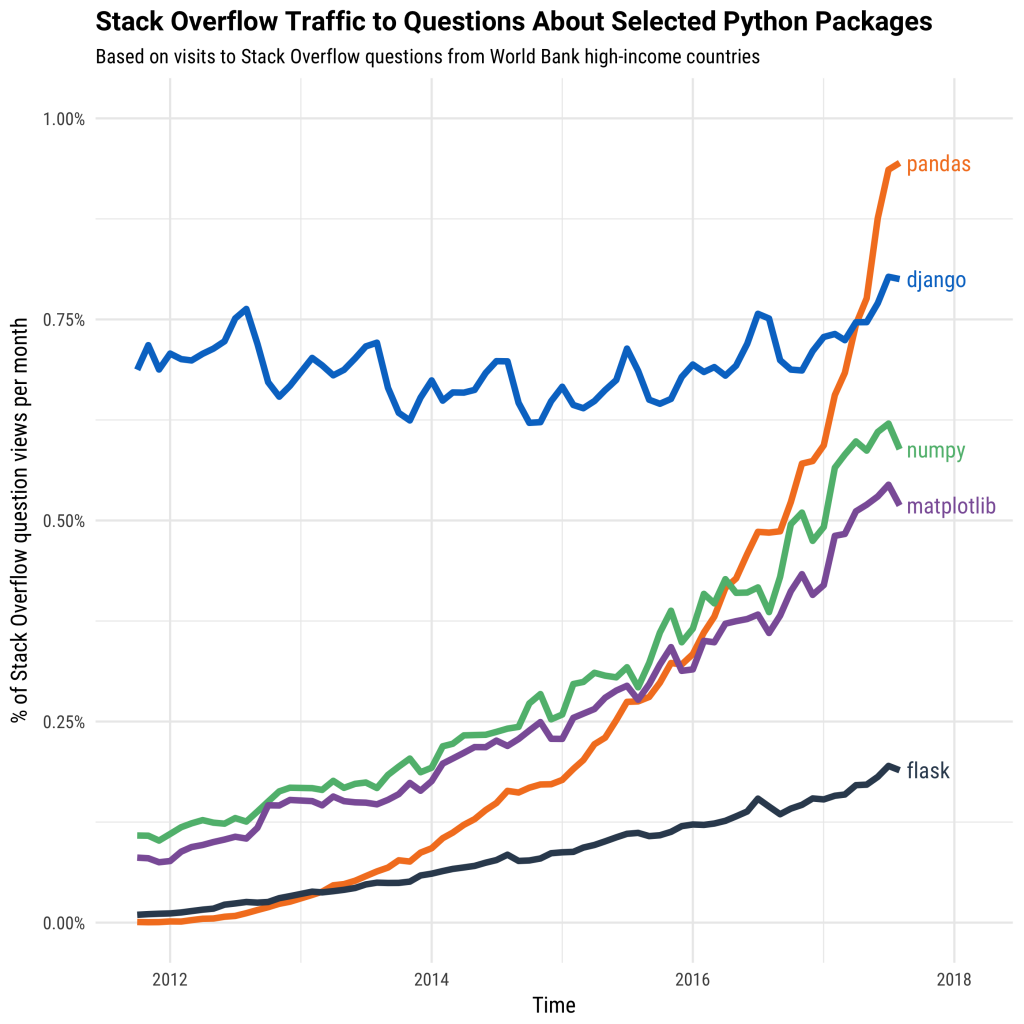
\includegraphics[width=0.7\textwidth]{numpy_grown.png}
\end{center}
\end{center}
\end{frame}

\begin{frame}[label={sec:org227d41f}]{Rendimiento de Python}
\begin{block}{¿Pero Python no era lento?}
Python por defecto sí\footnote{\url{https://arogozhnikov.github.io/2015/01/06/benchmarks-of-speed-numpy-vs-all.html}}

\begin{table}[htbp]
\caption{Tiempo de un benchmark (s)}
\centering
\begin{tabular}{lr}
\hline
Versión & Tiempo (ms)\\
\hline
Python puro & 183\\
Numpy & 5.97\\
Cython normal & 7.76\\
Cython optimizado & 2.18\\
Cython llamando a C & 2.22\\
\hline
\end{tabular}
\end{table}
\end{block}
\end{frame}


\begin{frame}[label={sec:org3c07bb0}]{Rendimiento de Python}
\begin{block}{¿Pero Python no era lento?\textsuperscript{\ref{org71116df}}}
\begin{table}[htbp]
\caption{tiempo matriz de distancias}
\centering
\begin{tabular}{ll}
\hline
Versión & Tiempo\\
\hline
Python & 9.51 seg\\
Naive numpy & 64.7 ms\\
Numba & 6.72 ms\\
Cython & 6.57 ms\\
Parakeet & 12.3 ms\\
Cython & 6.57 ms\\
\hline
\end{tabular}
\end{table}
\end{block}
\end{frame}

\begin{frame}[label={sec:org547194d}]{Rendimiento en Python}
\begin{itemize}
\item Procesar 1 GB de datos de Datos 
\begin{itemize}
\item 145.232 filas y 1.936 variables.
\end{itemize}

\item Comparando Python vs Scala (Java)\footnote{\url{https://stackoverflow.com/questions/32464122/spark-performance-for-scala-vs-python}}:
\end{itemize}

\begin{block}{Usando Spark}
\begin{center}
\begin{tabular}{rll}
\hline
Nodos & Versión & Tiempo\\
\hline
3 & Scala & 250 s\\
3 & Python & 246 s\\
\hline
\end{tabular}
\end{center}
\end{block}
\end{frame}

\begin{frame}[label={sec:orge0c4007}]{Rendimiento en Python}
\begin{block}{Hay distintas alternativas}
\begin{description}
\item[{Librería numpy}] Equivalente a Matlab, optimizable con BLAS.

\item[{PyPy}] Intérprete JIT, en migración a Python3.

\item[{Cython}] Python compilado a C (Python + tipos).

\item[{Numba}] Compilación JIT.
\end{description}
\end{block}

\begin{block}{Y en paralelo}
\begin{description}
\item[{Paralelismo fácil}] Clusters, snakemake, Luigi.

\item[{Librerías paralelas}] Dask.

\item[{Big Data}] pyspark.

\item[{Librerías en GPU}] PyCUDA, PyTorch.
\end{description}
\end{block}
\end{frame}

\begin{frame}[label={sec:orge1a0ceb}]{Caso de ejemplo: Numpy + Pandas}
\begin{center}
\begin{center}

\includegraphics[width=.7\textwidth]{python_numpy.png}
\end{center}
\end{center}

\begin{block}{Numpy}
\begin{itemize}
\item Librería matricial potente.

\item Pandas, leer tablas de datos.
\end{itemize}
\end{block}
\end{frame}



\begin{frame}[fragile,label={sec:orgd4c8fa4}]{Numpy es rápida y potente}
 \begin{columns}
\begin{column}{0.5\columnwidth}
\begin{block}{Usando Python}
\lstset{language=Python,label= ,caption= ,captionpos=b,numbers=none}
\begin{lstlisting}
def disteuc(xs,ys):
    sum = 0

    for x, y in zip(xs, ys):
        sum += (x-y)*(x-y)

    return sqrt(sum)

%time disteuc(xs,ys)
\end{lstlisting}
\end{block}
\end{column}

\begin{column}{0.5\columnwidth}
\begin{block}{Distancia euclídea con numpy}
\lstset{language=Python,label= ,caption= ,captionpos=b,numbers=none}
\begin{lstlisting}
def disteucnp(xs,ys):
    z = (xs-ys)
    return sqrt((z*z).sum())

%time disteucnp(xs,ys)
\end{lstlisting}
\end{block}
\end{column}
\end{columns}

\begin{block}{}
\scriptsize
CPU times: user 144 ms, sys: 0 ns, total: 144 ms
Wall time: 142 ms
\end{block}

\begin{block}{}
\scriptsize
CPU times: user 8 ms, sys: 0 ns, total: 8 ms
Wall time: 9.63 ms
\end{block}

{\color{blue}\href{https://docs.scipy.org/doc/numpy/user/quickstart.html}{https://docs.scipy.org/doc/numpy/user/quickstart.html}}
\end{frame}

\begin{frame}[label={sec:orgcaf244e}]{Pandas}
\begin{block}{Permite}
\begin{itemize}
\item Agrupar datos de distinto tipo.

\item Leer y escribir en csv, Excel.

\item Filtras y agrupar por ciertos atributos.
\end{itemize}
\end{block}

\begin{exampleblock}{Algunos ejemplo}
\begin{itemize}
\item DataSets de propinas.

\item DataSets del Titanic.

\item DataSets de nombres por años.
\end{itemize}
\end{exampleblock}

{\color{blue}\href{https://pandas.pydata.org/pandas-docs/stable/10min.html}{https://pandas.pydata.org/pandas-docs/stable/10min.html}}
\end{frame}

\begin{frame}[label={sec:org0ba850b}]{Visualizando \footnote{\url{https://bit.ly/2sUHcJu}}}
\begin{block}{Múltiples librerías}
\begin{description}
\item[{Matplotlib}] Librería por defecto, basada en Matlab.

\item[{Seaborn}] Sobre matplotlib, estilos.

\item[{Pandas}] Directamente.

\item[{Bokeh}] Gráficas webs.

\item[{Holoviews}] Sobre Bokeh, mayor nivel abstracción.

\item[{Altair}] Enfoque declarativo, web, en desarrollo.
\end{description}
\end{block}
\end{frame}

\begin{frame}[label={sec:orgdc87d67}]{Visualizando}
\begin{alertblock}{¿Qué aporta?}
\begin{itemize}
\item Excel ya me permite hacer gráficas.
\item Excel ya gestiona tablas.
\end{itemize}
\end{alertblock}

\begin{block}{Qué ofrece Python}
\begin{itemize}
\item Obtener datos de fuentes distintas

\item Análisis de datos visualmente

\item Diagramas interactivos
\end{itemize}
\end{block}
\end{frame}


\begin{frame}[label={sec:orgedd088a}]{Qué ofrece Python}
\begin{block}{Obtener datos de fuentes distintas}
\begin{itemize}
\item Redes sociales.
\item Páginas webs (\emph{web scraping}).
\item Otros recursos (Bases de Datos, \ldots{}).
\end{itemize}
\end{block}

\begin{block}{Análisis de datos visualmente}
\begin{itemize}
\item Interactivo: Notebook.

\item Forma declarativa.
\end{itemize}
\end{block}

\begin{block}{Diagramas interactivos}
\begin{itemize}
\item Explorar datos.
\item Panel de control interactivo.
\end{itemize}
\end{block}
\end{frame}


\begin{frame}[fragile,label={sec:org5759b16}]{Ejemplo: Caso de estudio}
 \begin{block}{Vamos a ver un ejemplo}
\begin{description}
\item[{Altair}] Librería en contrucción declarativa.

\item[{Objetivo}] Explorar tiempo de Seattle.
\end{description}
\end{block}

\begin{block}{Datos}
\lstset{language=Python,label=orgfd9d42b,caption= ,captionpos=b,numbers=none}
\begin{lstlisting}
df.head()
\end{lstlisting}
\scriptsize
\lstset{language=sh,label= ,caption= ,captionpos=b,numbers=none}
\begin{lstlisting}
date        precipitation  temp_max  temp_min  wind  weather
2012-01-01            0.0      12.8       5.0   4.7  drizzle
2012-01-02           10.9      10.6       2.8   4.5     rain
2012-01-03            0.8      11.7       7.2   2.3     rain
2012-01-04           20.3      12.2       5.6   4.7     rain
2012-01-05            1.3       8.9       2.8   6.1     rain
\end{lstlisting}
\end{block}
\end{frame}

\begin{frame}[fragile,label={sec:org7acd747}]{Precipitaciones por mes}
 \begin{block}{Código}
\begin{center}
\lstset{language=Python,label= ,caption= ,captionpos=b,numbers=none}
\begin{lstlisting}
alt.Chart(df).mark_line().encode(
    alt.X("date:T", timeUnit="month"),
    alt.Y("average(precipitation)")
)
\end{lstlisting}
\end{center}
\end{block}
\begin{center}
\begin{center}
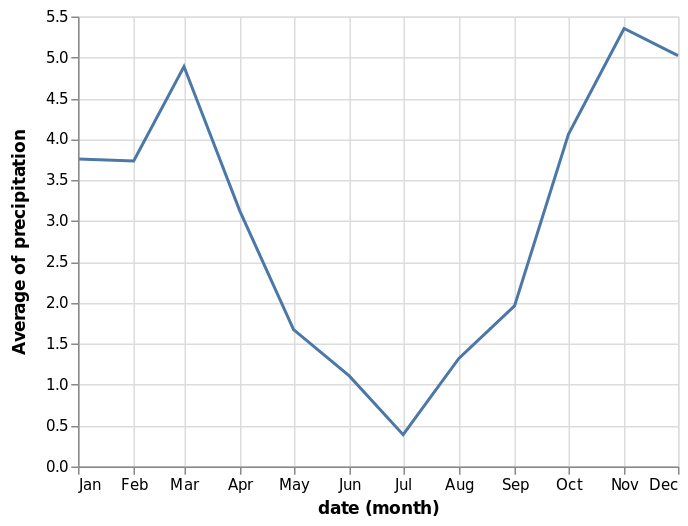
\includegraphics[width=0.6\textwidth]{seattle2.png}
\end{center}
\end{center}
\end{frame}

\begin{frame}[fragile,label={sec:org40a1c82}]{Precipitaciones por año y mes}
 \begin{block}{Código}
\begin{center}
\lstset{language=Python,label= ,caption= ,captionpos=b,numbers=none}
\begin{lstlisting}
alt.Chart(df).mark_line().encode(
    alt.X("date:T", timeUnit="yearmonth"),
    alt.Y("max(temp_max)"),
)
\end{lstlisting}
\end{center}
\end{block}
\begin{center}
\begin{center}
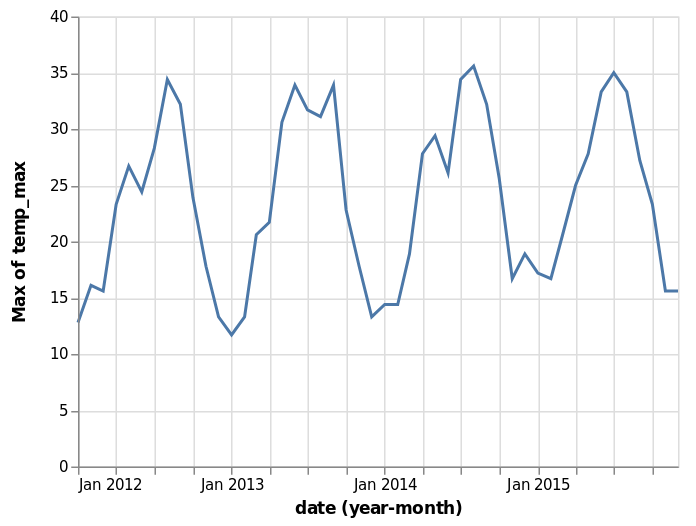
\includegraphics[width=0.6\textwidth]{seattle3.png}
\end{center}
\end{center}
\end{frame}

\begin{frame}[fragile,label={sec:orgaf2cbb6}]{Tipo de día}
 \begin{block}{Código}
\begin{center}
\lstset{language=Python,label= ,caption= ,captionpos=b,numbers=none}
\begin{lstlisting}
alt.Chart(df).mark_bar().encode(
    x=alt.X("date:N", timeUnit="month"),
    y="count()", color=alt.Color("weather",
    legend=alt.Legend(title="Weather type"), scale=scale),
)
\end{lstlisting}
\end{center}
\end{block}
\begin{center}
\begin{center}
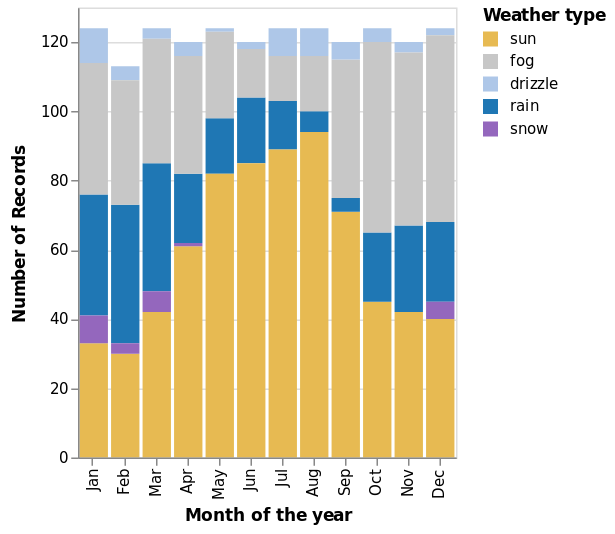
\includegraphics[width=0.5\textwidth]{seattle5.png}
\end{center}
\end{center}
\end{frame}


\begin{frame}[label={sec:org6e0bd8e}]{Demo de diagrama interactivo}
\begin{center}
\href{https://demo.bokehplots.com/apps/stocks}{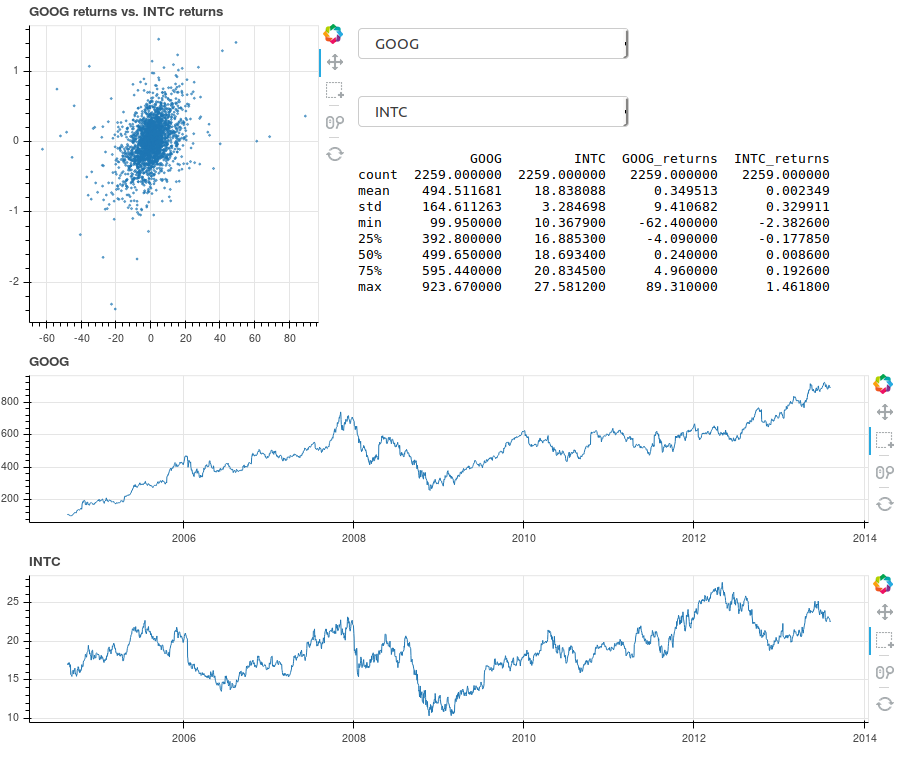
\includegraphics[width=0.8\textwidth]{./bokeh_demo1.png}}
\end{center}
\end{frame}

\begin{frame}[label={sec:org070532c}]{Demo de diagrama interactivo}
\begin{center}
\href{https://demo.bokehplots.com/apps/gapminder}{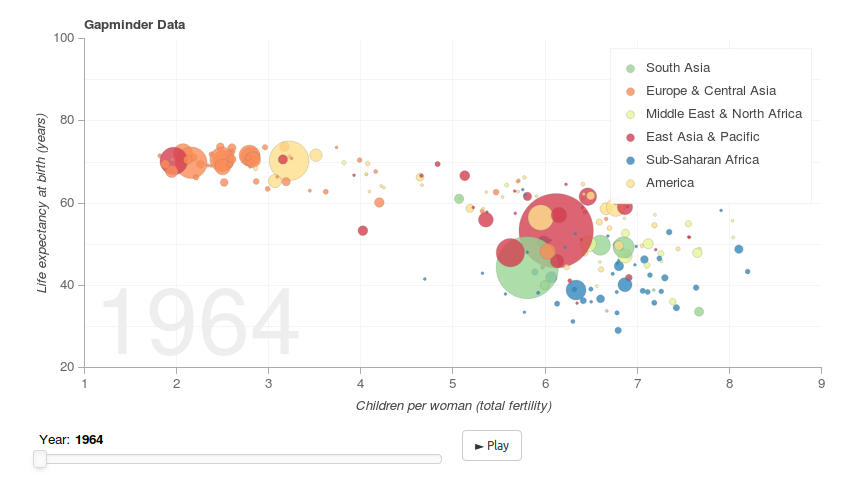
\includegraphics[width=0.8\textwidth]{./bokeh_demo2.png}}
\end{center}
\end{frame}





\section{Python y la programación web}
\label{sec:org8c1446d}

\begin{frame}[label={sec:org003f507}]{Python y la programación web}
\begin{columns}
\begin{column}{0.3\columnwidth}
\begin{center}
\begin{center}

\includegraphics[width=\textwidth]{django.png}
\end{center}
\end{center}
\end{column}
\begin{column}{0.7\columnwidth}
\begin{block}{Django}
\begin{itemize}
\item Entorno web Python más popular.

\item Inspirado en \alert{Rails} pero más explícito.

\item Muy integrado.
\end{itemize}
\end{block}
\end{column}
\end{columns}

\begin{columns}
\begin{column}{0.3\columnwidth}
\begin{center}
\begin{center}

\includegraphics[width=\textwidth]{flask.png}
\end{center}
\end{center}
\end{column}
\begin{column}{0.7\columnwidth}
\begin{block}{Flask}
\begin{itemize}
\item Entorno web más sencillo.

\item Menos funcionalidad, extensible.

\item Menos funcionalidad.
\end{itemize}
\end{block}
\end{column}
\end{columns}
\end{frame}


\begin{frame}[fragile,label={sec:org88ab399}]{Programa en Flask}
 \begin{exampleblock}{Ejemplo: hello world}
\lstset{language=Python,label= ,caption= ,captionpos=b,numbers=none}
\begin{lstlisting}
from flask import Flask
app = Flask(__name__)

@app.route("/")
def hello():
    return "Hello World!"

if __name__ == "__main__":
    app.run()
\end{lstlisting}
\end{exampleblock}

\begin{block}{Ejecutándolo}
\lstset{language=sh,label= ,caption= ,captionpos=b,numbers=none}
\begin{lstlisting}
$ python ejemplos/web.py
 * Running on http://127.0.0.1:5000/ (Press CTRL+C to quit)
\end{lstlisting}
\end{block}
\end{frame}

\begin{frame}[fragile,label={sec:orgfd76996}]{Cómo funciona}
 \begin{block}{Asignar}
\begin{enumerate}
\item \alert{@app.route} permite asociar una URL una función.
\item La función devuelve el resultado como respuesta de la URL.
\end{enumerate}
\end{block}

\begin{block}{Parámetros}
\begin{itemize}
\item La función puede recibir parámetros pasados por la URL.

\item Notación: <nombre>.
\end{itemize}
\end{block}

\begin{exampleblock}{Ejemplo de parámetro}
\lstset{language=Python,label= ,caption= ,captionpos=b,numbers=none}
\begin{lstlisting}
@app.route("/saluda/<name>")
def hello(name):
    return "Hola {}".format(name)
\end{lstlisting}
\end{exampleblock}
\end{frame}

\begin{frame}[fragile,label={sec:org90ab09f}]{Se puede combinar}
 \begin{exampleblock}{Ejemplo}
\lstset{language=Python,label= ,caption= ,captionpos=b,numbers=none}
\begin{lstlisting}
@app.route("/")
@app.route("/index")
def index():
  print("Pagina principal")
\end{lstlisting}
\end{exampleblock}

\begin{exampleblock}{Otro ejemplo}
\lstset{language=Python,label= ,caption= ,captionpos=b,numbers=none}
\begin{lstlisting}
@app.route("/saluda/<name>")
@app.route("/saluda")
def hello(name="desconocido"):
    return "Hola {}".format(name)
\end{lstlisting}
\end{exampleblock}
\end{frame}

\begin{frame}[label={sec:org2ade2d0}]{Templates}
\begin{block}{Plantilla}
\begin{itemize}
\item La salida suele ser código HTML complejo.
\item Se usa CSS personalizado (usando Bootstrap o similar).
\item El diseñador crea la plantilla.
\item La plantilla es HTML con referencias a variables (sintaxis especial).
\item El programa Python carga la plantilla y sustituye los valores de variables.
\end{itemize}
\end{block}

\begin{block}{}
Vamos a seguir con el ejemplo.
\end{block}
\end{frame}

\begin{frame}[fragile,label={sec:orga01c260}]{Flask con Template}
 \begin{block}{templates/index.html}
\lstset{language=HTML,label= ,caption= ,captionpos=b,numbers=none}
\begin{lstlisting}
<html>
    <head>
        <title>{{ title }} - Prueba</title>
    </head>
    <body>
        <h1>Saludos, {{ user.username }}!</h1>
    </body>
</html>
\end{lstlisting}
\end{block}

\begin{exampleblock}{Código}
\lstset{language=Python,label= ,caption= ,captionpos=b,numbers=none}
\begin{lstlisting}
from flask import render_template
from app import app

@app.route("/")
def index():
    user = {"username": "Miguel"}
    return render_template("index.html", title="Home", 
                           user=user)
\end{lstlisting}
\end{exampleblock}
\end{frame}

\begin{frame}[fragile,label={sec:org4a9d252}]{Lógica en la plantilla}
 \begin{block}{Plantilla: template/blog.html}
\lstset{language=HTML,label= ,caption= ,captionpos=b,numbers=none}
\begin{lstlisting}
<html>
    <head>
        
        <title>{{ title }}</title>
        
        <title>Bienvenido</title>
        
    </head>
    <body>
        <h1>Saludos, {{ user.username }}!</h1>
        
        <div><p>{{ post.author }}: <b>{{ post.body }}</b></p></div>
        
    </body>
</html>
\end{lstlisting}
\end{block}
\end{frame}

\begin{frame}[fragile,label={sec:org35db88a}]{Lógica en la plantilla}
 \begin{exampleblock}{Controlador}
\lstset{language=Python,label= ,caption= ,captionpos=b,numbers=none}
\begin{lstlisting}
from flask import render_template
from app import app

@app.route('/')
@app.route('/index')
def index():
    user = {'username': 'Miguel'}
    posts = [
        {
            'author': {'username': 'John'},
            'body': 'Beautiful day in Portland!'
        },
        {
            'author': {'username': 'Susan'},
            'body': 'The Avengers movie was so cool!'
        }
    ]
    return render_template('index.html', title='Home', 
                           user=user, posts=posts)
\end{lstlisting}
\end{exampleblock}
\end{frame}

\begin{frame}[label={sec:orgd93160e}]{Flask/Django ofrece mucho más}
\begin{block}{Ofrece}
\begin{itemize}
\item Acceso a la Base de Datos.
\item Validación de formularios.
\item Soporte de peticiones REST.
\item Componentes: Calendario, Google Maps, \ldots{}
\item Y mucho más.
\end{itemize}
\end{block}

\begin{block}{Ejemplo real}
\begin{center}
{\color{blue}\href{https://tflsgo.herokuapp.com/}{https://tflsgo.herokuapp.com/}}
\end{center}
\end{block}
\end{frame}

\begin{frame}[label={sec:org578e073}]{Web Scraping}
\begin{block}{Web scraping}
\begin{itemize}
\item Implica descargar datos de la web.
\end{itemize}
\end{block}

\begin{block}{Vamos a ver un ejemplo real}
\url{http://www.eweb.unex.es/eweb/maeb2015/?Conferencia\_\_\_Sesiones\_Especiales}
\end{block}
\end{frame}

\begin{frame}[fragile,label={sec:org6c48712}]{Programa}
 \begin{exampleblock}{Main}
\lstset{language=Python,label= ,caption= ,captionpos=b,numbers=none}
\begin{lstlisting}

def main(url):
    m = re.search("(.*\.es)/(.*)", url)
    prefix = m.group(1)
    html = requests.get(url)
    doc = lxml.html.fromstring(html.text)
    links = doc.xpath("//a/@href")
    ss_links = [link for link in links 
                if "Sesiones_Especiales___S" in link]

    for pos, ss_link in enumerate(ss_links):
        extract_ss_info(append_prefix(prefix, ss_link), pos)


if __name__ == "__main__":
    urls = [
        "http://www.eweb.unex.es/eweb/maeb2015/?Conferencia___Sesiones_Especiales"
    ]
    for url in urls:
        main(url)
\end{lstlisting}
\end{exampleblock}
\end{frame}

\begin{frame}[fragile,label={sec:orgcc9b502}]{Programa}
 \begin{block}{Funciones}
\lstset{language=Python,label= ,caption= ,captionpos=b,numbers=none}
\begin{lstlisting}
def extract_ss_info(url, previous):
    ss = requests.get(url)
    ss.encoding = "utf-8"
    doc = lxml.html.fromstring(ss.text)
    titles = doc.xpath("//h3/span/text()")

    if titles:
        title = titles[0]
    else:
        title = doc.xpath("//h3/text()")[0]

    expected = "S{}.".format(previous + 1)
    titles = doc.xpath("//em[contains(text(),"Organizador")]")
    assert (len(titles) == 1)
    elem = titles[0].getparent()
    while elem.tag != "p":
        elem = elem.getparent()
    ul = elem.getnext()
    authors = [author.text_content() for author in ul.xpath("li")]
    info = [title]
\end{lstlisting}
\end{block}
\end{frame}

\begin{frame}[label={sec:orgee9da74}]{Resumiendo}
\begin{columns}
\begin{column}{0.5\columnwidth}
\begin{center}
\begin{center}

\includegraphics[width=.7\textwidth]{thanks.png}
\end{center}
\end{center}
\end{column}


\begin{column}{0.5\columnwidth}
\begin{block}{Conclusiones}
\begin{itemize}
\item Python es muy útil.

\item Sintaxis sencilla.

\item Librerías muy potentes.
\begin{itemize}
\item Menos código.
\end{itemize}

\item Programación divertida.
\end{itemize}
\end{block}
\end{column}
\end{columns}

\begin{center}
\begin{center}

\includegraphics[width=.7\textwidth]{pythonuser.jpg}
\end{center}
\end{center}
\end{frame}
\end{document}